\documentclass[aspectratio=169]{beamer}

%---------------------------
%       Beamer Cheat Sheet
%---------------------------
% https://www.cpt.univ-mrs.fr/~masson/latex/Beamer-appearance-cheat-sheet.pdf

%---------------------------
%       Set Theme and Colors
%---------------------------

\usetheme[width=.1\paperwidth]{Hannover}
% \setbeamertemplate{sidebar canvas right}[vertical shading][top=red,bottom=blue]

\definecolor{QESblue}{HTML}{8AD2ED}
\definecolor{QESdarkblue}{HTML}{187ca2}
\definecolor{QESlightblue}{HTML}{c4e8f6}

\setbeamercolor{sidebar}{bg=QESlightblue}
\setbeamercolor{titlelike}{fg=QESdarkblue}

\setbeamercolor{palette sidebar secondary}{fg=QESdarkblue}
\setbeamercolor{title in sidebar}{fg=QESdarkblue}
\setbeamercolor{author in sidebar}{fg=QESdarkblue}

\addtobeamertemplate{sidebar left}{}{\vfill \hspace{.006\paperwidth} 
\includegraphics[width=.08\paperwidth]{../../../logo.png} \vspace{.006\paperwidth} } 
% \addtobeamertemplate{sidebar left}{}{\vfill \hspace{.00001\paperwidth} 
\includegraphics[width=.093\paperwidth]{../../figures/qes-qr.png} \vspace{.003\paperwidth} } 

%---------------------------
%       No navigation symbols
%---------------------------
\setbeamertemplate{navigation symbols}{}

%---------------------------
%       Set Fonts
%---------------------------
\usepackage{helvet}
\renewcommand{\familydefault}{\sfdefault}
\usepackage{sansmathfonts}
\usepackage{upgreek}

\setbeamerfont{frametitle}{series=\bfseries, size=\Large}
\setbeamerfont{title in sidebar}{series=\bfseries, size=\small}
\setbeamertemplate{caption}{\it\raggedright\insertcaption\par}

%---------------------------
%       Math font packages
%---------------------------
\usepackage{dsfont, amsmath, amsthm, mathtools}
\usepackage{bbm, bm}
\usepackage[T1]{fontenc}
\usepackage[version=3]{mhchem}

%---------------------------
%       Figure packages
%---------------------------
\usepackage{graphicx}
\graphicspath{{../../figures}}

\usepackage{epstopdf}
\usepackage{color}

\setbeamerfont{caption}{size=\footnotesize}

\usepackage{subfigure}

%---------------------------
%       Manual placement packages
%---------------------------
\usepackage{tikz}
\usetikzlibrary{calc}

%---------------------------
%       Local Macros
%---------------------------

\newcommand{\manualpic}[4]{
    % inputs {filename}{figure options}{x offset}{y offset}
    \tikz[remember picture, overlay] \node[anchor=center] at ($(current page.center)+(#3,#4)$) {\includegraphics[#2]{#1}};
}

\newcommand{\manualtext}[3]{
    % inputs {text}{x offset}{y offset}
    \tikz[remember picture, overlay] \node[anchor=center] at ($(current page.center)+(#2,#3)$) {#1};
}

\newcommand{\manualtextleft}[3]{
    % inputs {text}{x offset}{y offset}
    \tikz[remember picture, overlay] \node[anchor=west] at ($(current page.center)+(#2,#3)$) {#1};
}

\newcommand{\manualtextright}[3]{
    % inputs {text}{x offset}{y offset}
    \tikz[remember picture, overlay] \node[anchor=east] at ($(current page.center)+(#2,#3)$) {#1};
}

\newcommand{\slidereference}[1]{
    \manualtextleft{\tiny #1}{-0.47\linewidth}{-0.47\textheight}
}

\newcommand{\dv}[2]{\frac{\mathrm{d}#1}{\mathrm{d}#2}}

\title{Future Climate}
\author{Timescales}

\begin{document}

\begin{frame}{Future Climate: Timescales}
    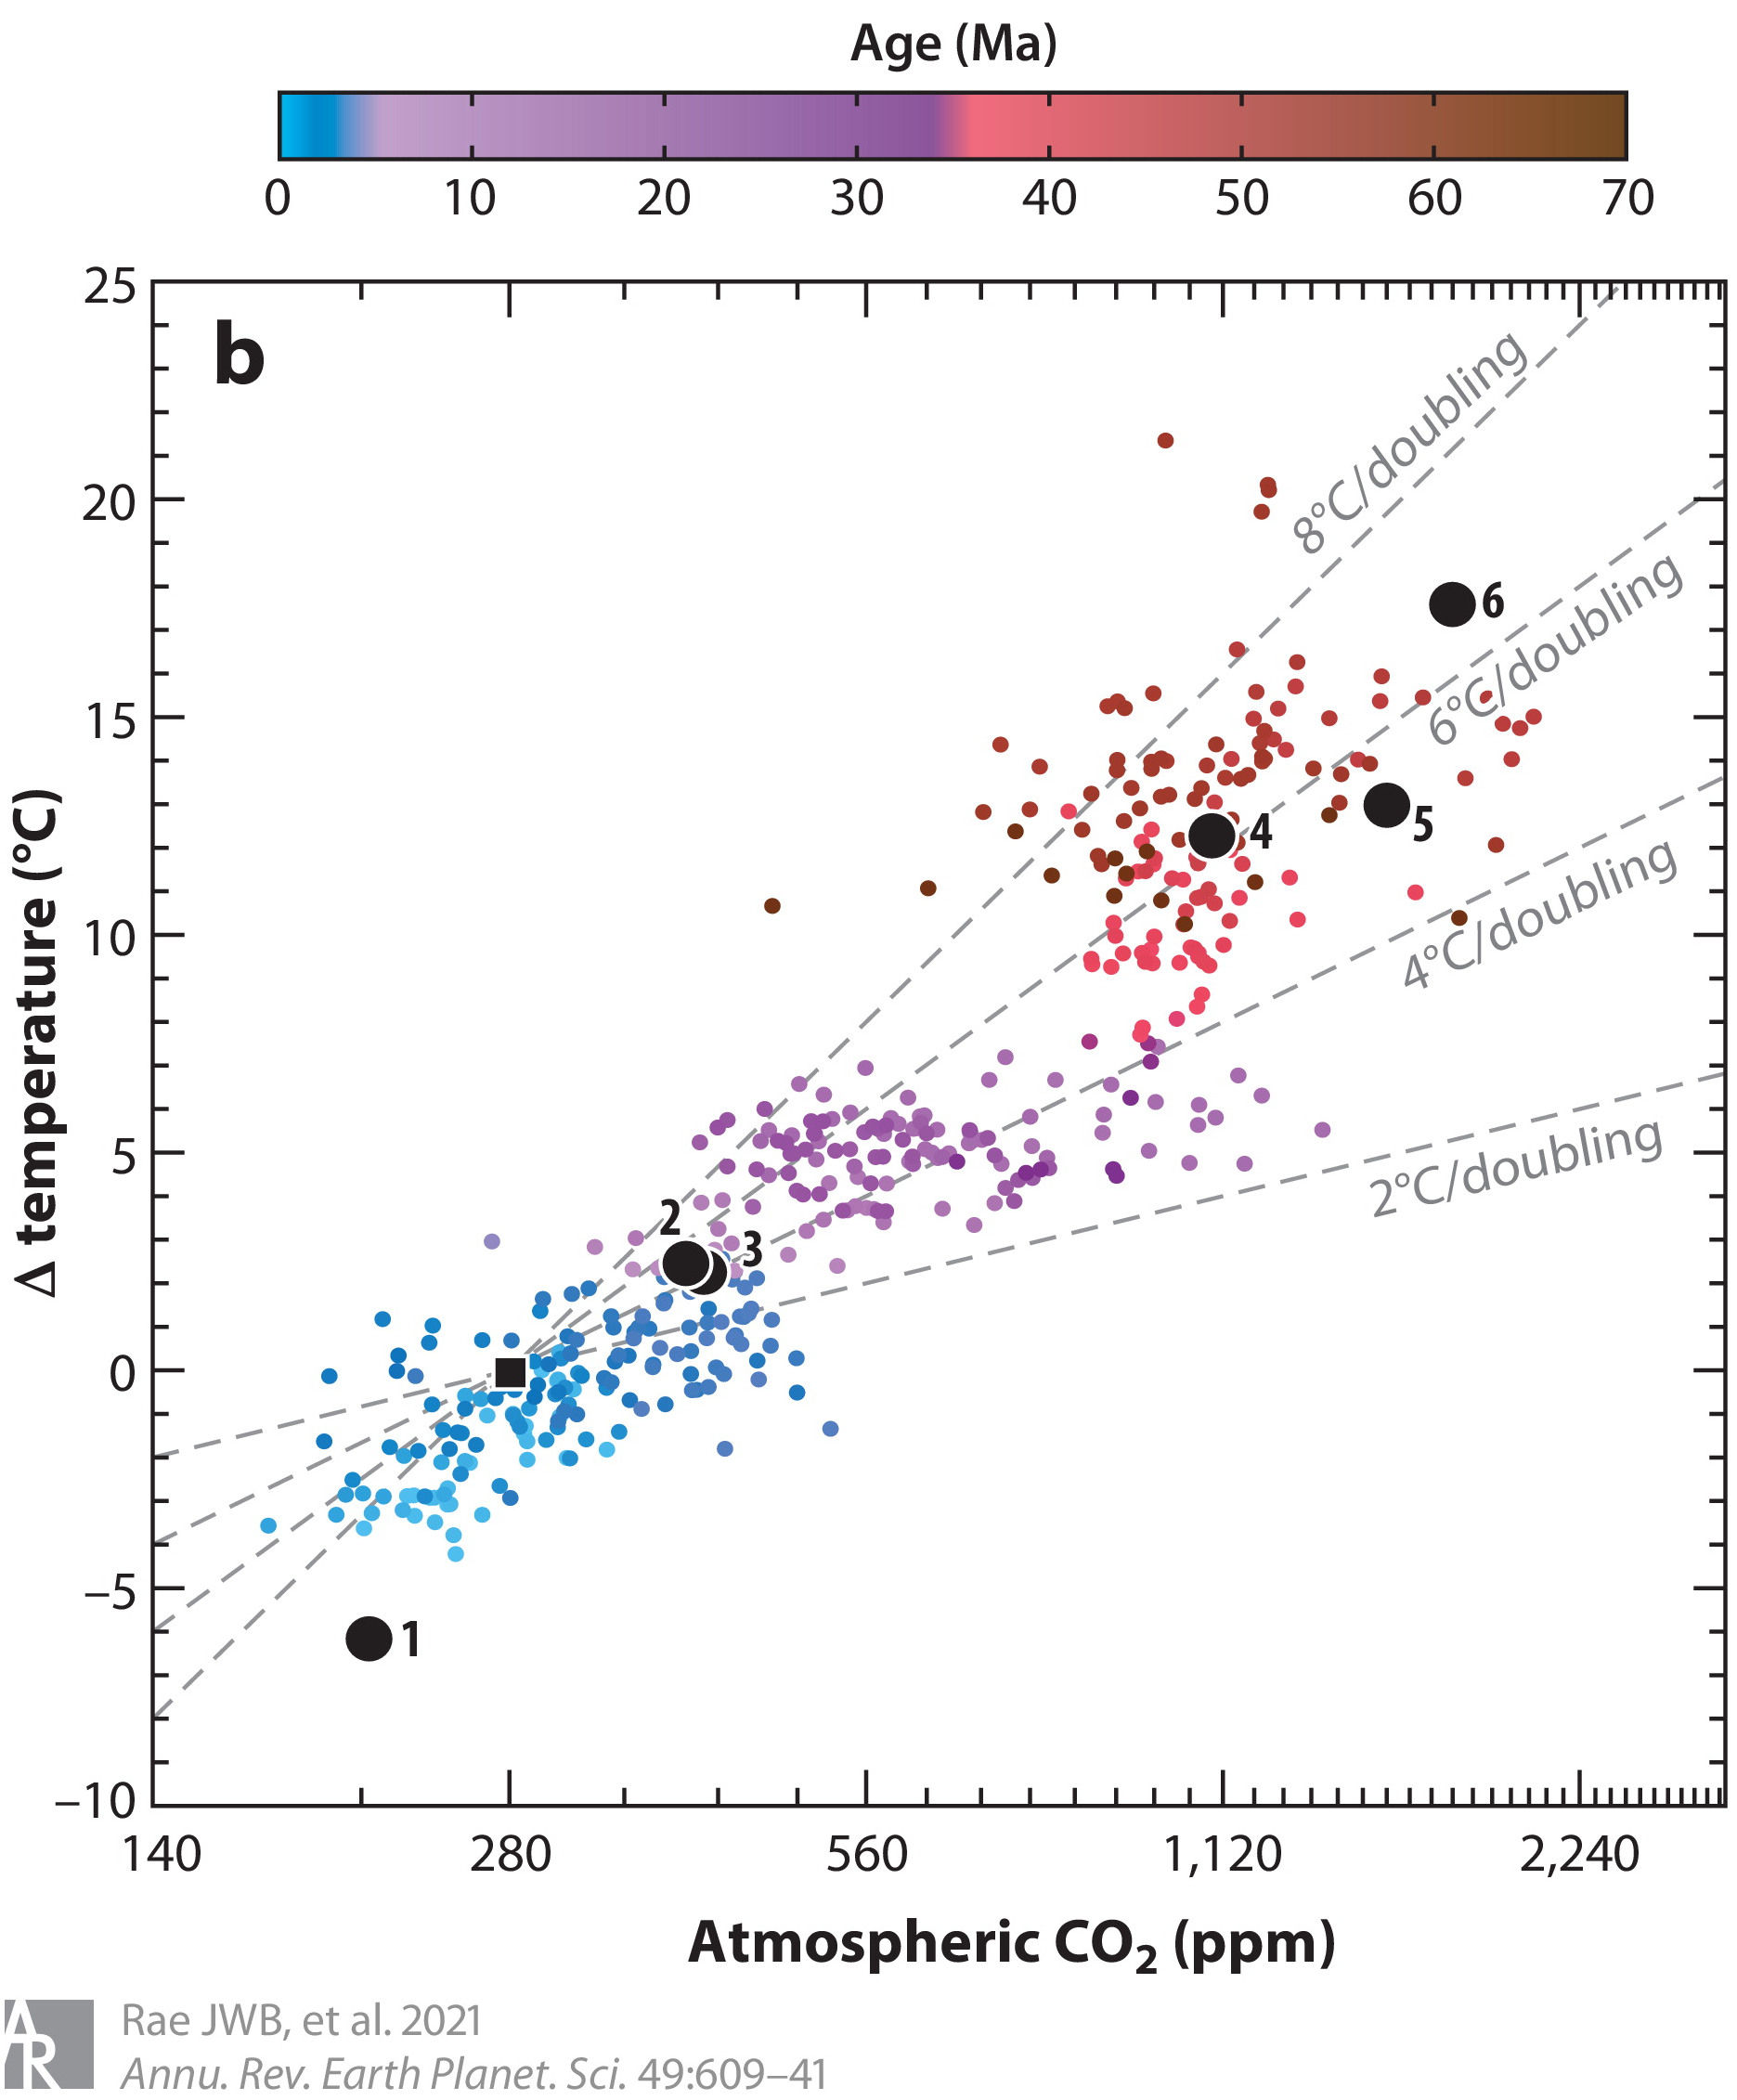
\includegraphics[width=\linewidth, totalheight=0.8\textheight, keepaspectratio]{future-palaeo-sensitivity.jpeg}
\end{frame}

\section{(Un)certainty}

\begin{frame}{(Un)certainty}

    % weather vs. climate - specific predictions hard; average predictions more certain

    % apparent linear relationship between cumulative emissions and temperature rise
    % https://www.ipcc.ch/report/ar6/wg1/figures/summary-for-policymakers/figure-spm-10

    % but what about feedbacks?
    % https://www.ipcc.ch/report/ar6/wg1/figures/summary-for-policymakers/figure-spm-7

\end{frame}

\section{Future Climate}

\begin{frame}{Commitments}
    % Transient Climate Response (TCR) vs. Equilibrium Climate Sensitivity (ECS)

    % IPCC comparison
    % https://www.ipcc.ch/report/ar6/wg1/figures/chapter-7/figure-7-18
 
    % https://archive.ipcc.ch/ipccreports/tar/wg1/345.htm#:~:text=The%20%EF%BF%BDtransient%20climate%20response,commitment%EF%BF%BD%20has%20been%20realised.


    % Graphical Illustration
    % https://external-preview.redd.it/IxOap0w7k967MDrOZURwHwW-M-S_jCN-G9_ntLvlSDQ.jpg?auto=webp&v=enabled&s=2aa3f076bab5683b00354bb3437d6a819d5e1e50

    % Use 4-box model!

    % released CO2 = more trapped energy = warming... but how much?
\end{frame}


\section{Climate Sensitivity}
% https://www.carbonbrief.org/explainer-how-scientists-estimate-climate-sensitivity/

\begin{frame}{Climate Sensitivity}
    % IPCC models estimates give a range
    % https://www.ipcc.ch/report/ar6/wg1/figures/chapter-7/faq-7-3-figure-1

    % But IPCC models are 'ground truthed' against the modern world... (narrow range of conditions, hindcast figure)    
    % Complex feedbacks (Alex's Fig)
\end{frame}

\begin{frame}{Precedent?}
    % we are pushing the climate into an unknown regime.
    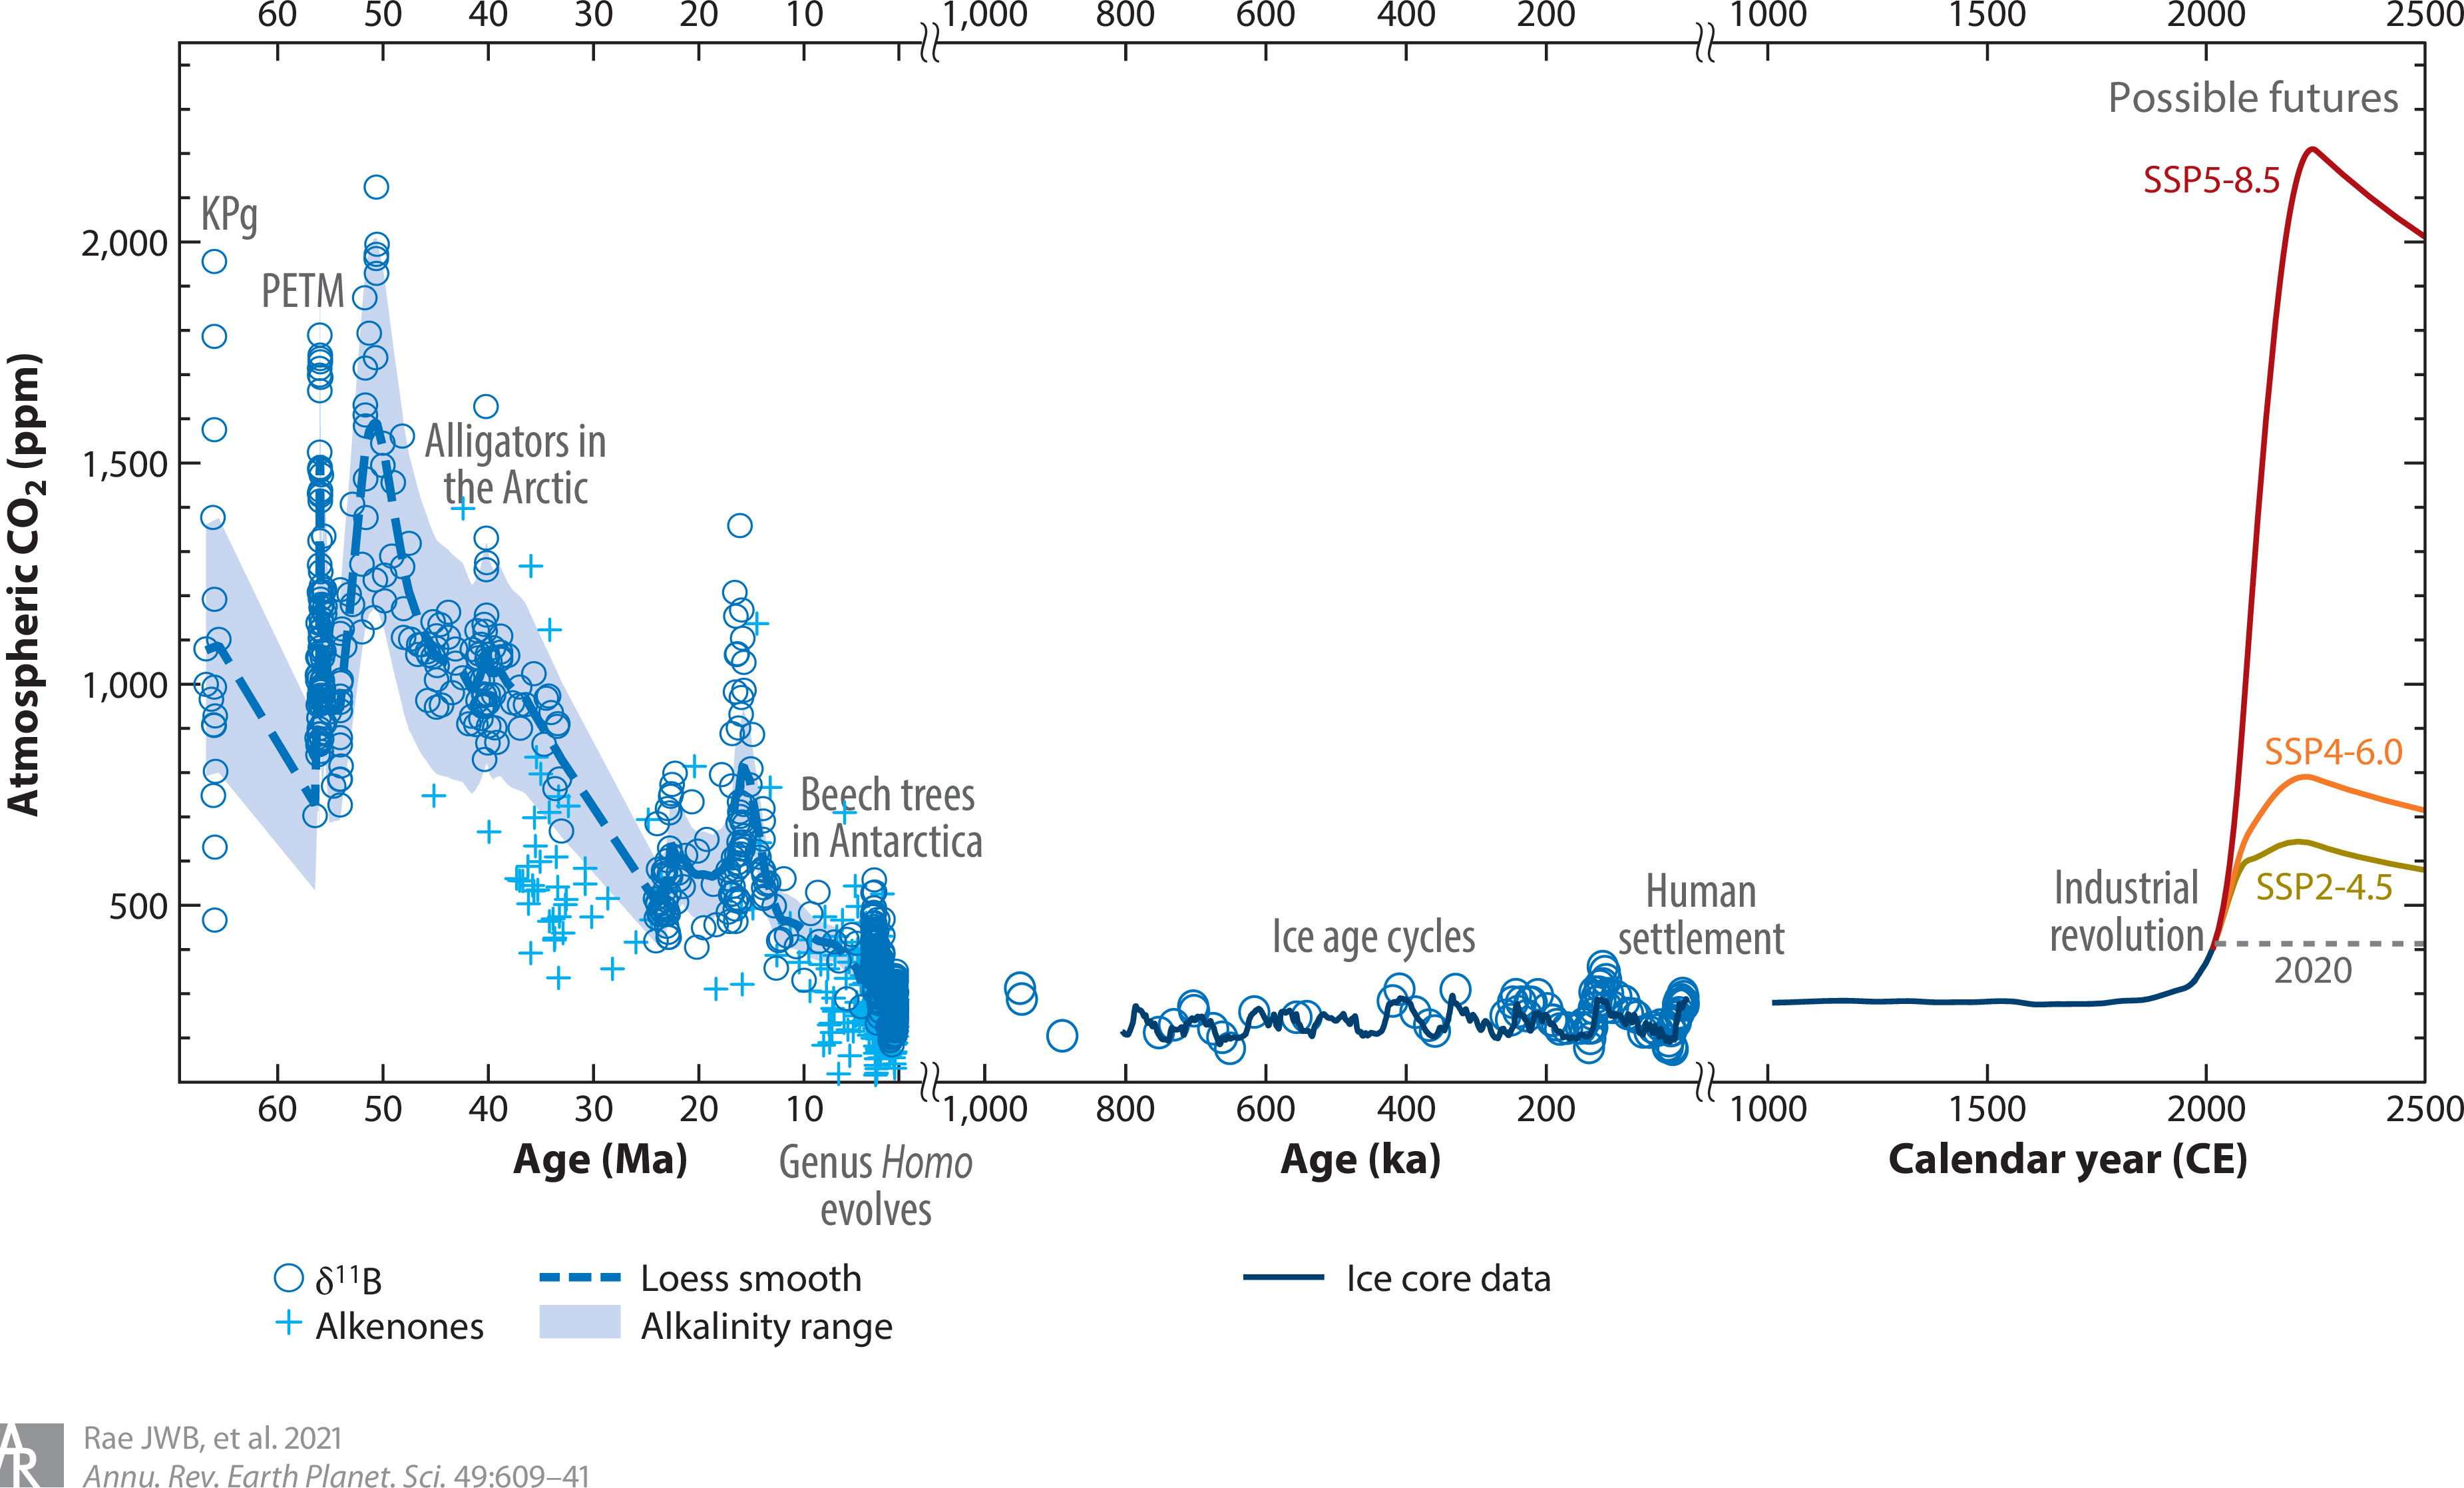
\includegraphics[width=\linewidth, totalheight=0.8\textheight, keepaspectratio]{future-palaeo-co2.jpeg}
\end{frame}            

\section{Past Climate}

\begin{frame}{Climate Records}
    % how do we know what happened in past climates?
    % palaeo-CO2 project
    % palaeo-temperature
\end{frame}

\begin{frame}{Estimates of Sensitivity}
    % palaeoclimate was more sensitive?
    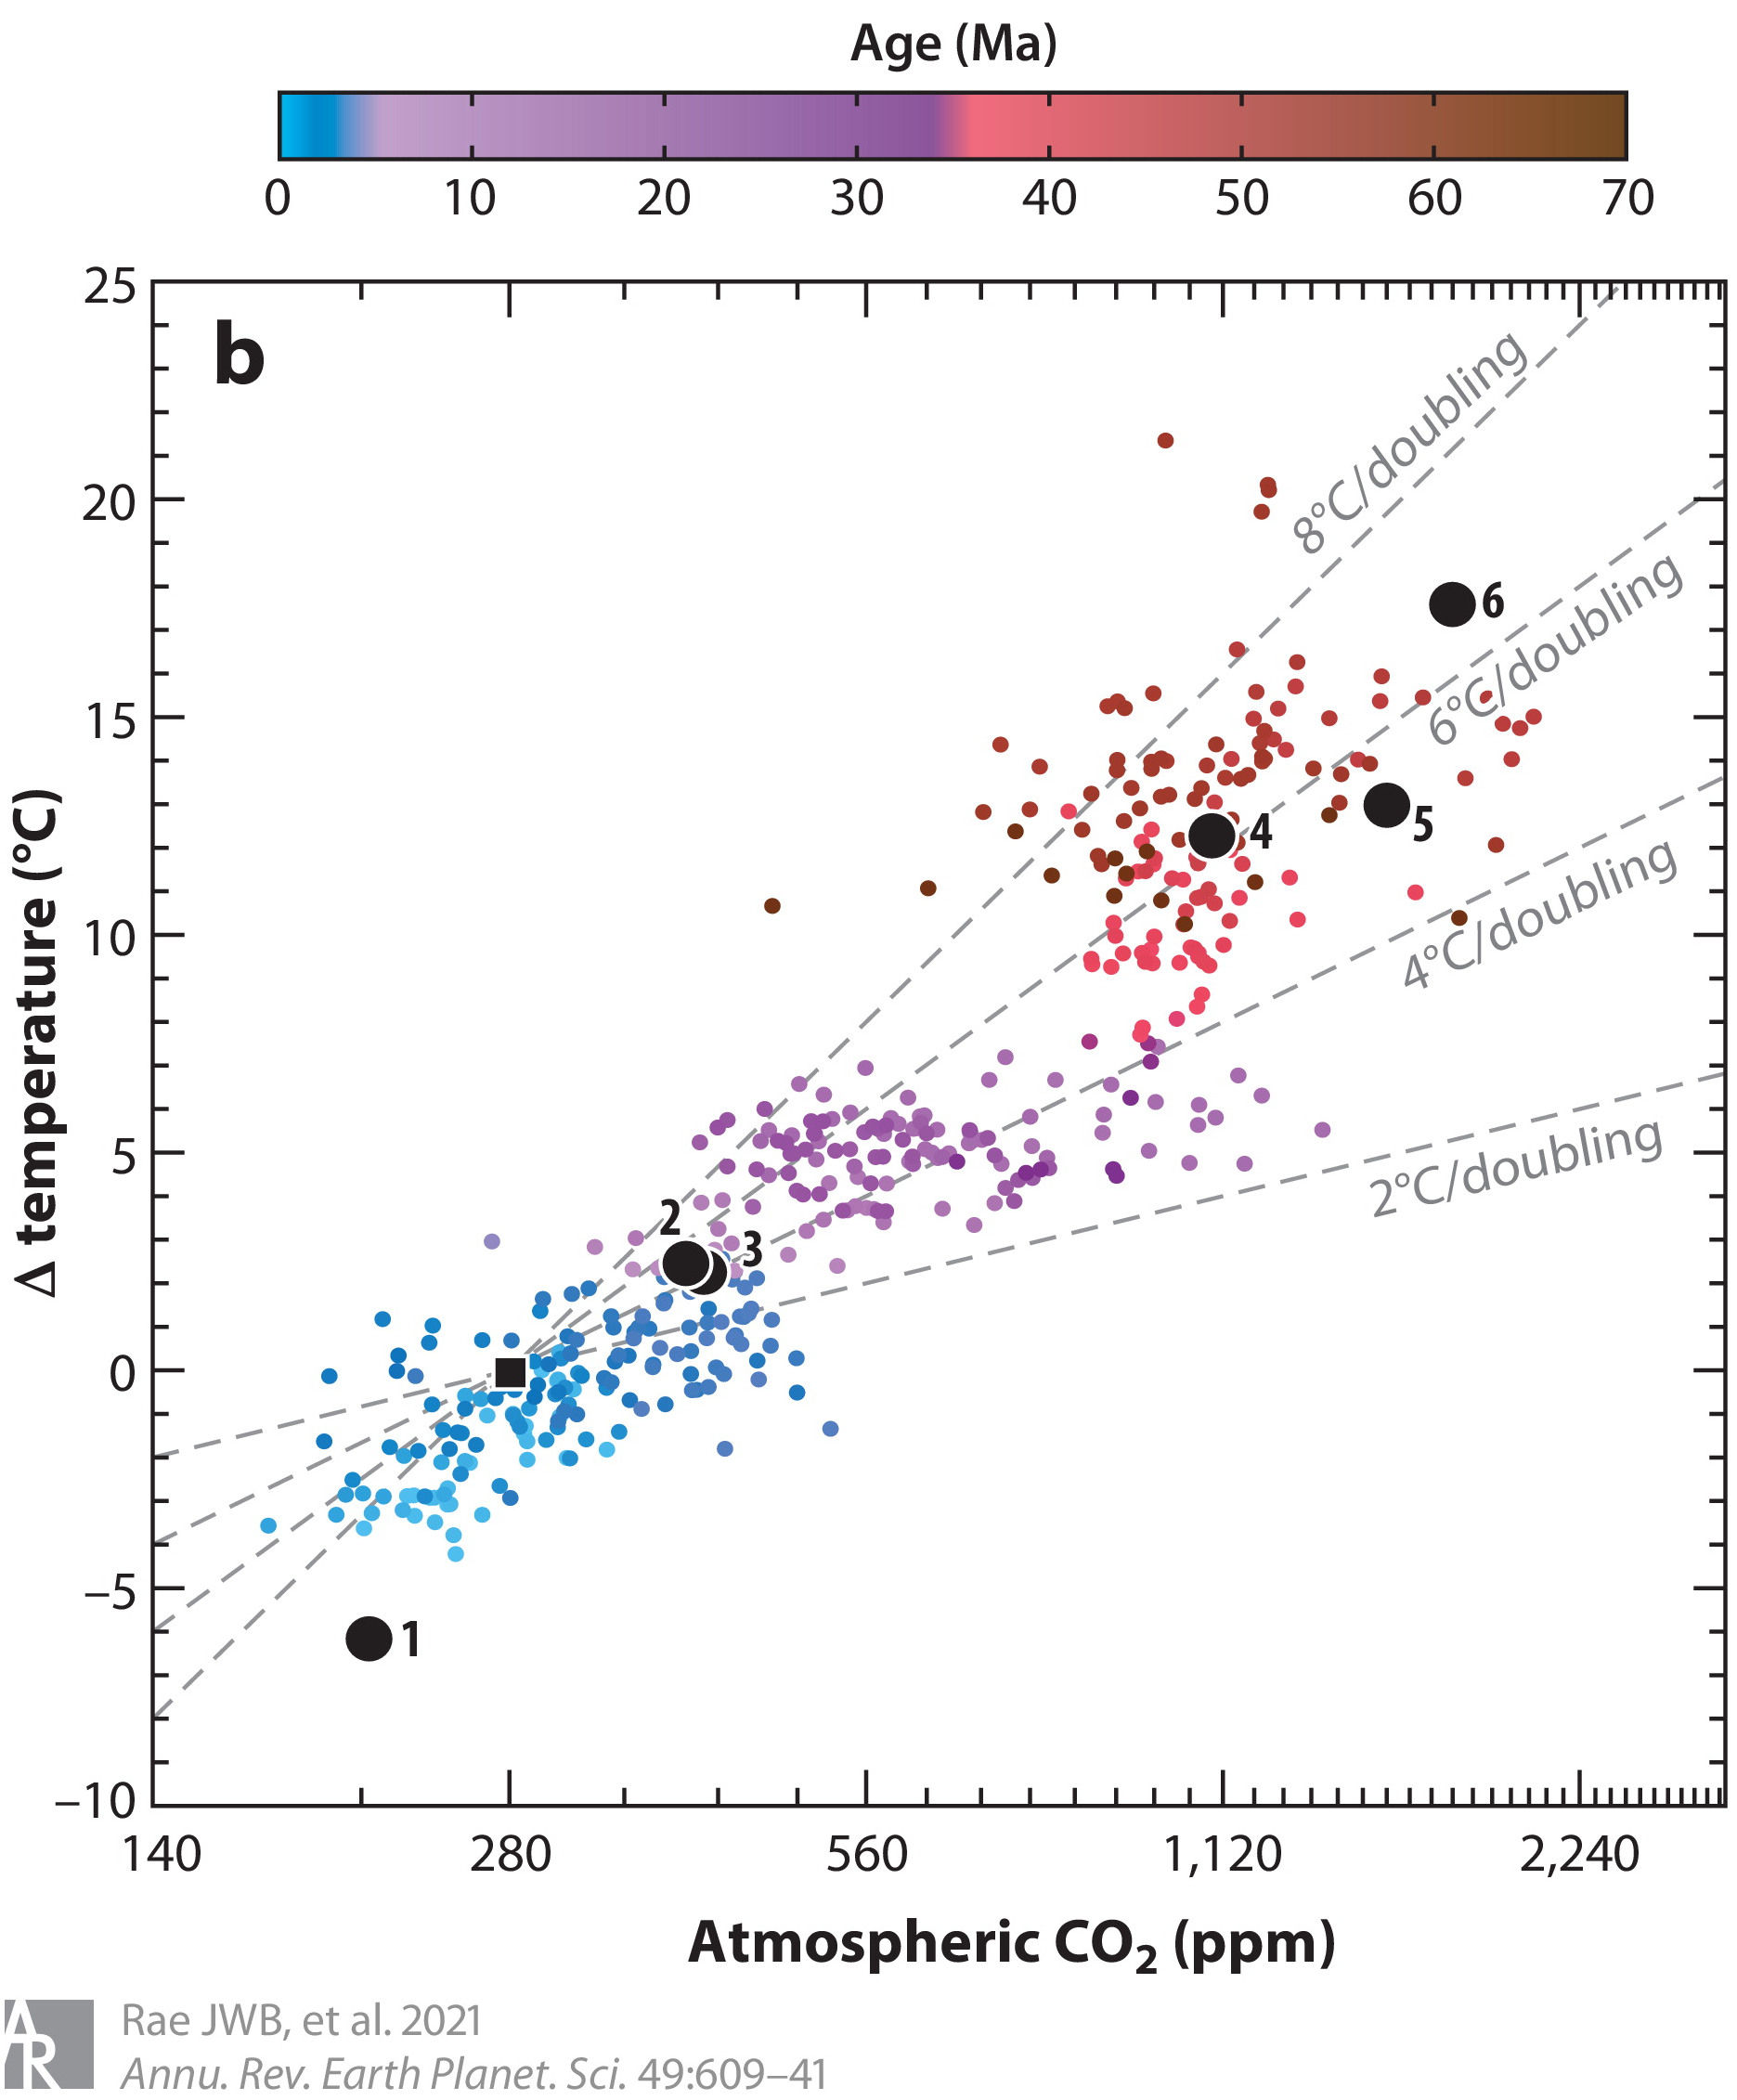
\includegraphics[width=\linewidth, totalheight=0.8\textheight, keepaspectratio]{future-palaeo-sensitivity.jpeg}
\end{frame}

\section{Recovery}

\begin{frame}{Timescales of Recovery}
    % PETM sediments
\end{frame}


\end{document}





% \begin{frame}{TITLE}
% \end{frame}